\documentclass[10pt]{article}
\usepackage[a4paper,margin=16mm,top=14mm,bottom=15mm]{geometry}
\usepackage{fontspec}
\setmainfont{Liberation Serif}
\setsansfont{Montserrat}
\usepackage{microtype}
\usepackage{booktabs}
\usepackage{tabularx}
\usepackage{array}
\usepackage{graphicx}
\usepackage{xcolor}
\usepackage{enumitem}
\usepackage{titlesec}
\usepackage{fancyhdr}
\usepackage{caption}
\usepackage{hyperref}

\definecolor{navy}{HTML}{183A59}
\definecolor{teal}{HTML}{287271}
\definecolor{lightblue}{HTML}{EEF4F7}
\definecolor{midgray}{HTML}{58636D}
\hypersetup{colorlinks=true,linkcolor=navy,urlcolor=teal}

\pagestyle{fancy}
\fancyhf{}
\fancyhead[L]{\sffamily\footnotesize Tabular foundation models under label scarcity}
\fancyhead[R]{\sffamily\footnotesize July 2026}
\fancyfoot[C]{\sffamily\footnotesize \thepage}
\renewcommand{\headrulewidth}{0.3pt}

\titleformat{\section}{\sffamily\bfseries\large\color{navy}}{}{0pt}{}
\titleformat{\subsection}{\sffamily\bfseries\normalsize\color{navy}}{}{0pt}{}
\titlespacing*{\section}{0pt}{6pt}{3pt}
\titlespacing*{\subsection}{0pt}{4pt}{2pt}
\setlength{\parindent}{0pt}
\setlength{\parskip}{3.5pt}
\setlist[itemize]{leftmargin=4.5mm,itemsep=1pt,topsep=2pt}
\newcolumntype{Y}{>{\raggedright\arraybackslash}X}
\newcommand{\method}[1]{\texttt{\small #1}}
\newcommand{\keybox}[1]{%
  \begin{center}
  \fcolorbox{navy}{lightblue}{\parbox{0.94\linewidth}{#1}}
  \end{center}}

\begin{document}

\begin{center}
{\sffamily\bfseries\LARGE\color{navy}
Tabular Foundation Models and Focused\\[-1mm]
Semi-Supervised Learning under Label Scarcity}

\vspace{2mm}
{\sffamily\large A controlled evaluation on ten OpenML classification datasets}

\vspace{1.5mm}
{\sffamily\small 960 new final-grid runs \quad|\quad balanced accuracy as the primary metric}
\end{center}
\vspace{-1mm}
\hrule
\vspace{3mm}

\section{Summary}

This study tested whether modern tabular foundation models and targeted
semi-supervised mechanisms improve prediction when only 50--500 labels are
available. TabPFN-3 and TabICLv2 were evaluated in their standard few-shot form,
then extended with self-training. Four trainable alternatives used the unlabeled
training pool through graph regularization, retrieval attention,
class-conditional representation alignment, or a combination of these
mechanisms.

\keybox{\textbf{Main result.} The two foundation models were the strongest and
most reliable methods in the focused study. TabICLv2 achieved mean balanced
accuracy 0.743 and TabPFN-3 0.739; their self-training variants reached 0.745
and 0.741. The gains from self-training were real but small and highly
selective. Among the trainable SSL methods, unlabeled retrieval attention was
best (0.668). Combining all regularizers did not improve on attention alone.}

Against six established benchmark comparators---CatBoost, XGBoost,
self-training LightGBM, VIME, SCARF, and SSLAE---a foundation-model variant was
best in 31 of the 40 dataset-by-budget cells. The result is not that unlabeled
data is uniformly beneficial: the strongest evidence is instead that frozen
foundation models already provide a difficult baseline, and a conservative
self-training guard can add small gains without broadly degrading it.

\section{Experimental design}

The benchmark used ten canonical OpenML datasets: phoneme, spambase,
MagicTelescope, adult, bank-marketing, electricity, satimage, segment,
steel-plates-fault, and jannis. Every method used the same predetermined split
for each dataset, seed, and label budget. The grid contained four budgets
(50, 100, 250, 500) and three seeds. Phase A evaluated two frozen foundation
models (240 runs); Phase C evaluated six SSL methods (720 runs). All 960 runs
completed successfully, with no missing or duplicate keys.

The protocol was inductive. Graphs, pseudo-labels, representation learning, and
retrieval memory used labeled and unlabeled \emph{training} rows only.
Validation labels were restricted to calibration, early stopping, and safe
fallback decisions. Test rows were introduced only as prediction queries.
TabPFN-3 and TabICLv2 used the native mixed-type pandas representation; the
trainable methods used the benchmark's established imputed, scaled, and
one-hot encoded representation. Accuracy, macro-F1, log-loss, ROC-AUC,
average precision where defined, Brier score, ECE, and runtime were retained
as secondary outcomes.

\section{What was implemented}

\small
\begin{tabularx}{\textwidth}{@{}p{40mm}Y@{}}
\toprule
\textbf{Method} & \textbf{Implementation used in the final grid}\\
\midrule
\method{tabpfn3} &
TabPFN 8.1.0 using the verified
\method{tabpfn-v3-classifier-v3\_default.ckpt}; labeled context only, native
feature view, ordered and validated class probabilities.\\
\method{tabiclv2} &
Pinned \method{tabicl-classifier-v2-20260212.ckpt}; labeled context only and
the same native-view, few-shot protocol.\\
\method{tabpfn3\_self\_training} and
\method{tabiclv2\_self\_training} &
One shared, deterministic engine with up to three hard pseudo-label rounds,
class-balanced confidence selection, per-class and total caps, validation-based
round selection, and fallback to the frozen predictor.\\
\method{laplacian\_ssl} &
Trainable encoder/classifier with a sparse training-only kNN graph, locally
scaled affinities, mini-batched Laplacian loss, ramp-up, validation stopping,
and collapse checks.\\
\method{unlabeled\_attention\_ssl} &
Trainable encoder with batched top-\(k\) retrieval and residual attention over
labeled and unlabeled training memory; self-neighbors and validation/test rows
were excluded.\\
\method{embedding\_alignment\_ssl} &
Confidence-weighted, class-conditional prototype attraction with inter-class
separation and representation-collapse diagnostics.\\
\method{geometric\_attention\_ssl} &
Modular combination of supervised loss, pseudo-label consistency, Laplacian
regularization, retrieval attention, prototype alignment, and class separation,
with confidence and loss ramp-up.\\
\bottomrule
\end{tabularx}
\normalsize

\newpage

\section{Results}

\begin{table}[h!]
\centering
\caption*{\sffamily\bfseries Complete-grid results for the eight requested methods}
\small
\begin{tabular}{@{}lrrrrr@{}}
\toprule
\textbf{Method} & \textbf{Bal. acc.} & \textbf{Mean rank} &
\textbf{Macro-F1} & \textbf{ECE} & \textbf{Time/run (s)}\\
\midrule
TabICLv2 + self-training & \textbf{0.745} & \textbf{2.44} & 0.747 & 0.045 & 11.1\\
TabICLv2                 & 0.743 & \textbf{2.44} & 0.745 & 0.044 & 6.3\\
TabPFN-3 + self-training & 0.741 & 2.74 & 0.743 & 0.040 & 13.3\\
TabPFN-3                 & 0.739 & 2.91 & 0.741 & \textbf{0.039} & 8.8\\
Unlabeled attention      & 0.668 & 5.03 & 0.657 & 0.122 & 5.0\\
Laplacian SSL            & 0.617 & 6.40 & 0.602 & 0.099 & 7.6\\
Combined model           & 0.596 & 6.92 & 0.569 & 0.082 & 9.5\\
Embedding alignment      & 0.583 & 7.12 & 0.559 & 0.111 & 3.6\\
\bottomrule
\end{tabular}
\vspace{1mm}

\parbox{0.94\linewidth}{\footnotesize
Means pool 120 successful runs per method. Mean rank first averages the three
seeds within each of the 40 dataset-by-budget cells and then ranks methods
within each cell; lower is better. ECE is expected calibration error.}
\end{table}

\begin{figure}[h!]
\centering
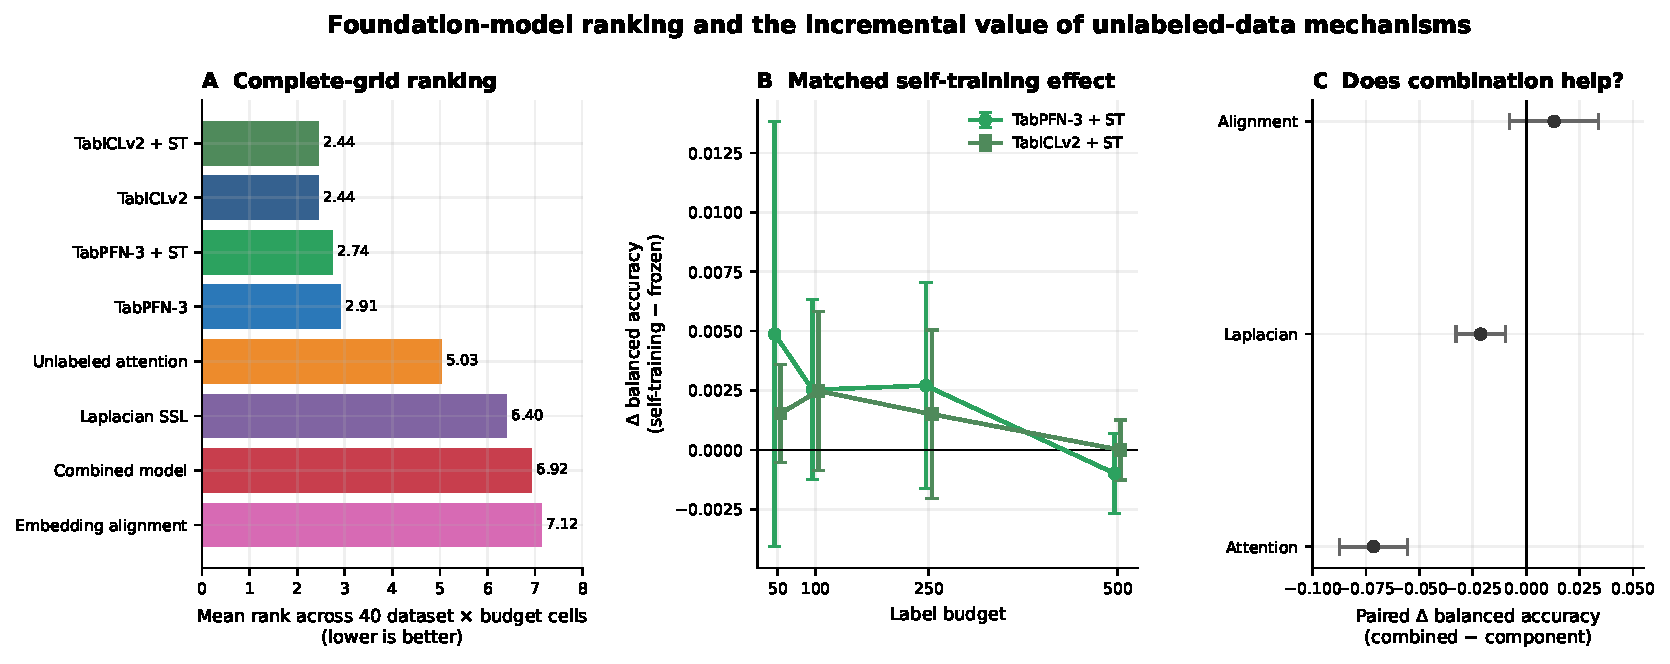
\includegraphics[width=\textwidth]{summary_figure.pdf}
\caption*{\footnotesize
\textbf{A:} failure-aware ranking over the requested methods.
\textbf{B:} exact paired self-training effects; bars are descriptive 95\%
intervals across matched dataset/seed cells.
\textbf{C:} the combined model compared with separately trained components on
identical run keys.}
\end{figure}

\subsection{Foundation models and self-training}

TabICLv2 was slightly stronger than TabPFN-3: the exact paired difference
TabPFN-3 minus TabICLv2 was \(-0.0048\) balanced accuracy (descriptive 95\%
interval \(-0.0092,-0.0003\)). Self-training increased mean balanced accuracy
by \(+0.0014\) for TabICLv2 and \(+0.0023\) for TabPFN-3. These averages hide
how conservative the mechanism was. The selected prediction was identical to
the frozen model in 83/120 TabICLv2 cells and 86/120 TabPFN-3 cells; positive
changes occurred in only 23 and 20 cells, respectively. The largest consistent
benefit occurred on steel-plates-fault, with smaller gains on bank-marketing.
At 500 labels, neither backbone showed a mean benefit.

The foundation-model family won 31/40 cells when compared with the six key
historical baselines. Pooled balanced accuracy was 0.722 for CatBoost, 0.712
for XGBoost, 0.690 for SSLAE, 0.687 for SCARF, 0.686 for VIME, and 0.675 for
self-training LightGBM. These are benchmark-level comparisons rather than
claims of statistical dominance on every dataset.

\subsection{Trainable SSL mechanisms}

Unlabeled attention was the strongest trainable SSL method and won three cells
within the focused eight-method grid, including adult at budgets 100 and 250.
Its mean attention mass was 96\% on unlabeled memory, confirming that the final
registration genuinely used the unlabeled pool. Laplacian SSL was modestly
better than historical label propagation (\(+0.014\), interval crossing zero)
but worse than label spreading (\(-0.064\)). Embedding alignment was not
competitive as a standalone predictor.

The full combined model improved on embedding alignment by \(+0.013\) on
average, but underperformed Laplacian SSL by \(-0.021\) and unlabeled attention
by \(-0.072\). More regularization therefore did not translate into better
generalization.

\newpage

\section{Reliability, diagnostics, and interpretation}

\subsection{Repair of the combined model}

An early segment run collapsed to exactly chance performance (\(1/7\) balanced
accuracy). The failure was reproduced before Phase C and traced to retrieval
composition: because the unlabeled pool was much larger, an unrestricted
top-\(k\) search could fill every memory slot with unlabeled examples. Class
mapping, output dimension, and probability ordering were verified separately.
The repair introduced deterministic balanced retrieval from labeled and
unlabeled memory, batched full-pool diagnostics, supervised warm-up, and
confidence/loss ramp-up. A final 12-cell segment/Jannis gate passed before the
full attention-family grid was submitted.

Across the final grid, no method triggered a representation-collapse flag and
no attention memory contained validation or test rows. The combined model
maintained effective embedding rank 32 and allocated mean attention mass 55\%
to labeled and 45\% to unlabeled neighbors. It nevertheless triggered 21/120
constant-prediction warnings; Laplacian SSL triggered 17/120. These warnings
were retained rather than filtered because their probabilities were finite and
the runs satisfied the prespecified operational checks. They help explain why
stable optimization did not guarantee competitive accuracy.

The sparse graphs contained about 21,000 training nodes and 53,000 edges on
average and took 1.7 seconds to construct. The foundation models were also the
best calibrated methods (mean ECE 0.039--0.045), while trainable SSL ECE ranged
from 0.082 to 0.122. Average runtime per final run ranged from 3.6 seconds for
alignment to 13.3 seconds for TabPFN-3 self-training. For context, historical
SSLAE, SCARF, and VIME runs averaged 57, 177, and 263 seconds.

\section{What can and cannot be concluded}

\begin{itemize}
\item \textbf{Supported:} under this label-budget protocol, TabPFN-3 and
TabICLv2 are stronger overall than the focused trainable SSL implementations
and the selected historical baselines.
\item \textbf{Supported:} validation-guarded TFM self-training is safe and can
produce small gains, but most cells revert to the frozen model and the benefit
largely disappears at 500 labels.
\item \textbf{Supported:} retrieval attention is the most promising trainable
unlabeled-data mechanism in this study; combining all mechanisms is not
beneficial.
\item \textbf{Not supported:} a general claim that unlabeled data helps every
method. The trainable SSL grid did not include a final-source-hash supervised
encoder control for every architecture, so its results are benchmark
comparisons rather than pure causal estimates of unlabeled-data value.
\end{itemize}

Three seeds permit matched descriptive uncertainty but not strong significance
claims for small differences. CPU RAM and reliable peak-GPU-memory summaries
were not serialized. Post-training oracle pseudo-label accuracy,
neighbor-label purity, and class-prior drift were also not consistently
available as analysis fields. Average precision is undefined for the
multiclass tasks and was left missing rather than imputed.

\section{Conclusion}

The practical result is straightforward: use a frozen tabular foundation model
as the primary low-label baseline, with conservative self-training as an
optional refinement. TabICLv2 was marginally strongest overall; TabPFN-3 was
very close and slightly better calibrated. If a trainable SSL alternative is
needed, retrieval attention is the best candidate from this study. The
Laplacian, prototype-alignment, and complete combined variants add complexity
without improving the final ranking.

\section{Reproducibility}

All 240 Phase-A and 720 Phase-C shards were validated before aggregation. The
final test suite passed 25 tests with one skipped. Canonical results,
machine-readable paired effects, figures, source/configuration hashes,
checkpoint identities, Slurm metadata, and the full technical report are
preserved under \method{results/reports/bar\_ilan\_tfm\_ssl\_final/}. The
historical 17-method result file was not modified.

\vfill
\hrule
\vspace{1.5mm}
{\footnotesize\sffamily
Primary metric: balanced accuracy. Values in this brief were generated from
the validated canonical result tables; no model was selected or altered after
test evaluation.}

\end{document}
